% FEATURE: should be defined in intro chapter

\subsection{Motivation}

%this section shall give a clear motivation (making tacit knowledge explicit)/some application examples (analysis (some example questions, see Berger et al. for motivation of these questions), communication, knowledge managament/transfer), include the FODA notation and show FeatureIDE examples (without analysis)
%=> how do we get from ad-hoc to our vision?

\subsection{Features in Online Configurators}

\subsection{Dependencies Between Features}

% \subsection{Features in Industrial Practice}

% better: Excel table of products or features/dependencies

% give some experience reports/motivation from practice (Berger et al)

% (maybe mention Marlin case study about Feature Location?)

% \subsection{Feature Models and Configurations}

% even better: show examples of structured configuration processes (eg. subway, Linux)

% then define feature model + configuration and give examples

\subsection{Feature Diagrams} % syntax, notation, visuals

\begin{frame}{~}
show running example as a feature diagram with cross-tree-constraints

explain notation (formal semantics later)

discuss pros/cons

show diagram in some established tools: FeatureIDE, pure::variants

FMs describe features and their dependencies explicitly - tease (in)valid configurations (interaction?)
\end{frame}

% TODO move?
%\subsection{Implicit Knowledge About Features}
%
%usually, features + constraints are not modeled explicitly (tacit knowledge / lost in code) => pros/cons










\subsection{Software Product Lines} % todo: recap from intro lecture. up to now: only variants.
\begin{frame}{\insertsubsection\ \mytitlesource{\fospl}}
	\leftorright{
		\mydefinition{Mass Customization}{
			\begin{itemize}
				\item opposed to mass production
				\item opposed to individual customization
				\item idea: produce customized goods as efficient as with mass production
			\end{itemize}
		}
		\href{https://commons.wikimedia.org/wiki/File:Geely_assembly_line_in_Beilun,_Ningbo.JPG}{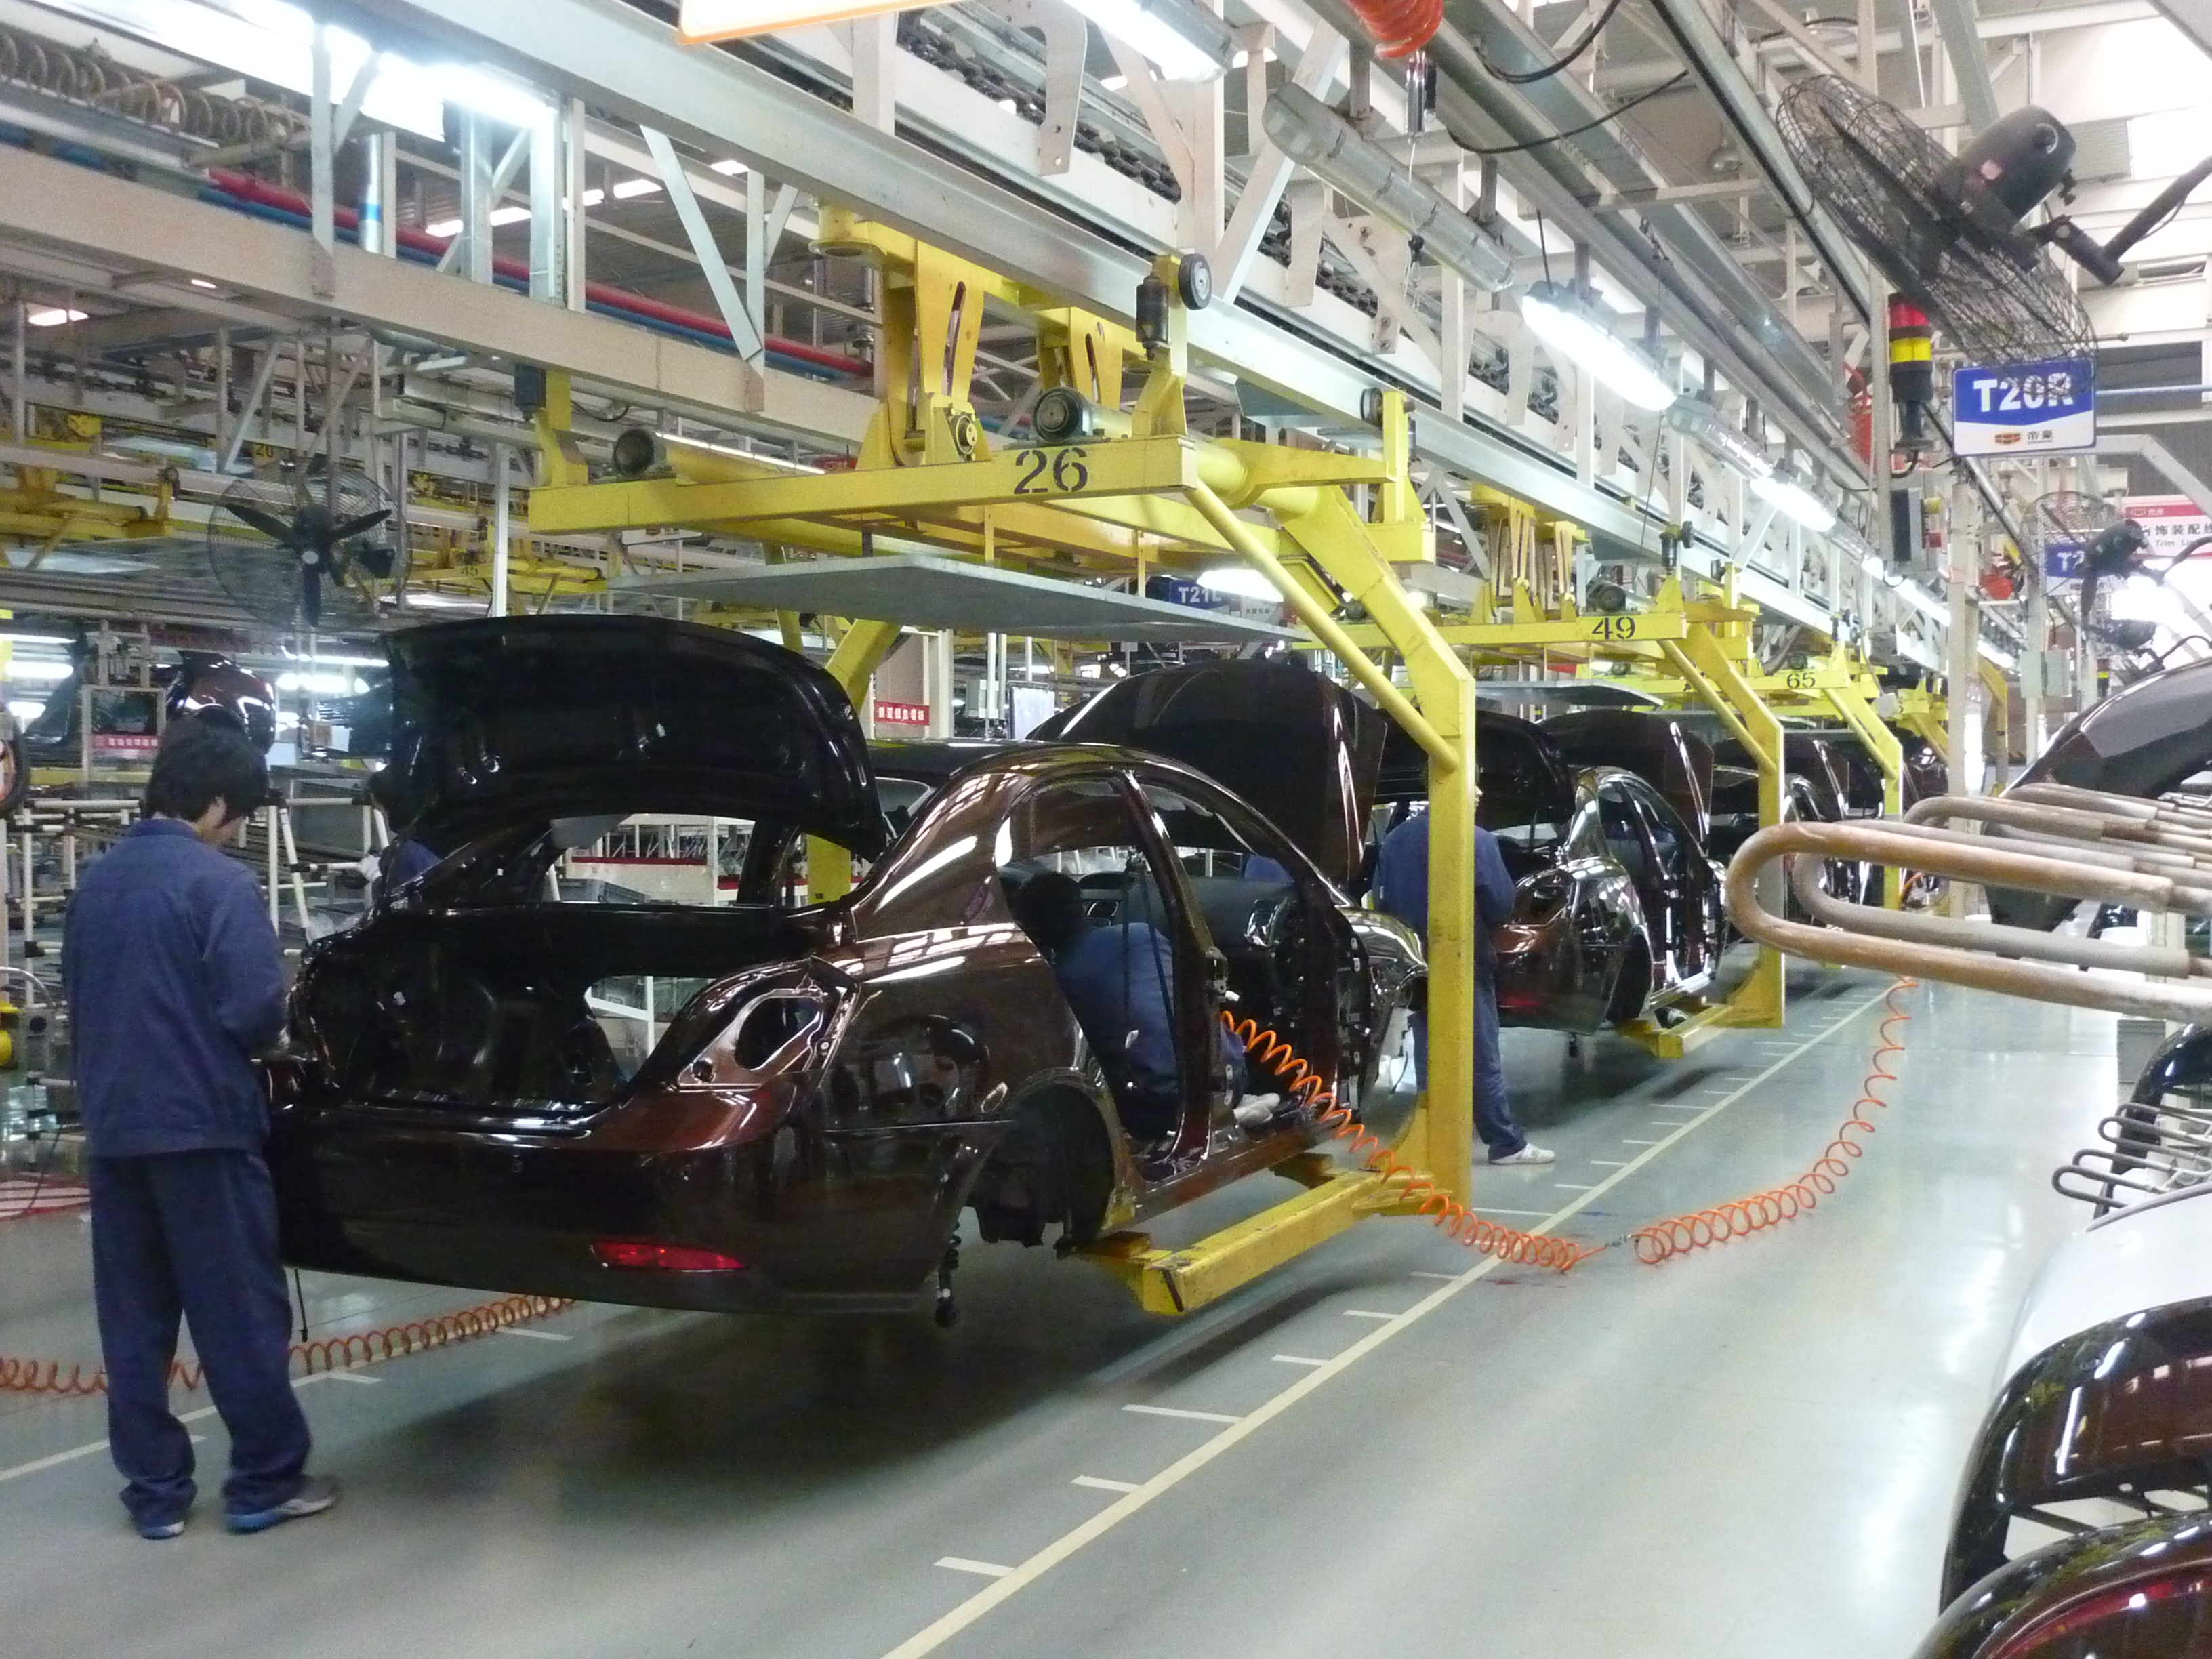
\includegraphics[width=\linewidth,trim=0 50 0 240,clip]{car-manufacturing}}
	}{
		\mydefinition{Software Product Line}{
			\begin{itemize}
				\item set of software-intensive systems (aka. products)
				\item sharing a common, managed set of features
				\item satisfying the needs of a domain
				\item developed from a common set of core assets (reuse)
			\end{itemize}
		}
		\mydefinition{Feature}{ % todo: examples
			\begin{itemize}
				\item domain abstraction
				\item used for communication by stakeholders (e.g., manager, developer, tester, customer, marketing)
				\item specifies differences between products
			\end{itemize}
		}
	}
\end{frame}

%todo : scoping

% motivation for dependencies between features
\xkcd{2369}{BE5c-26s} % paper processor 25s

\subsection{Dependencies Between Features}
\begin{frame}{\insertsubsection}
	\partofpage{70}{\myexampletight{Thomas Configuring a Notebook}{\only<1,3->{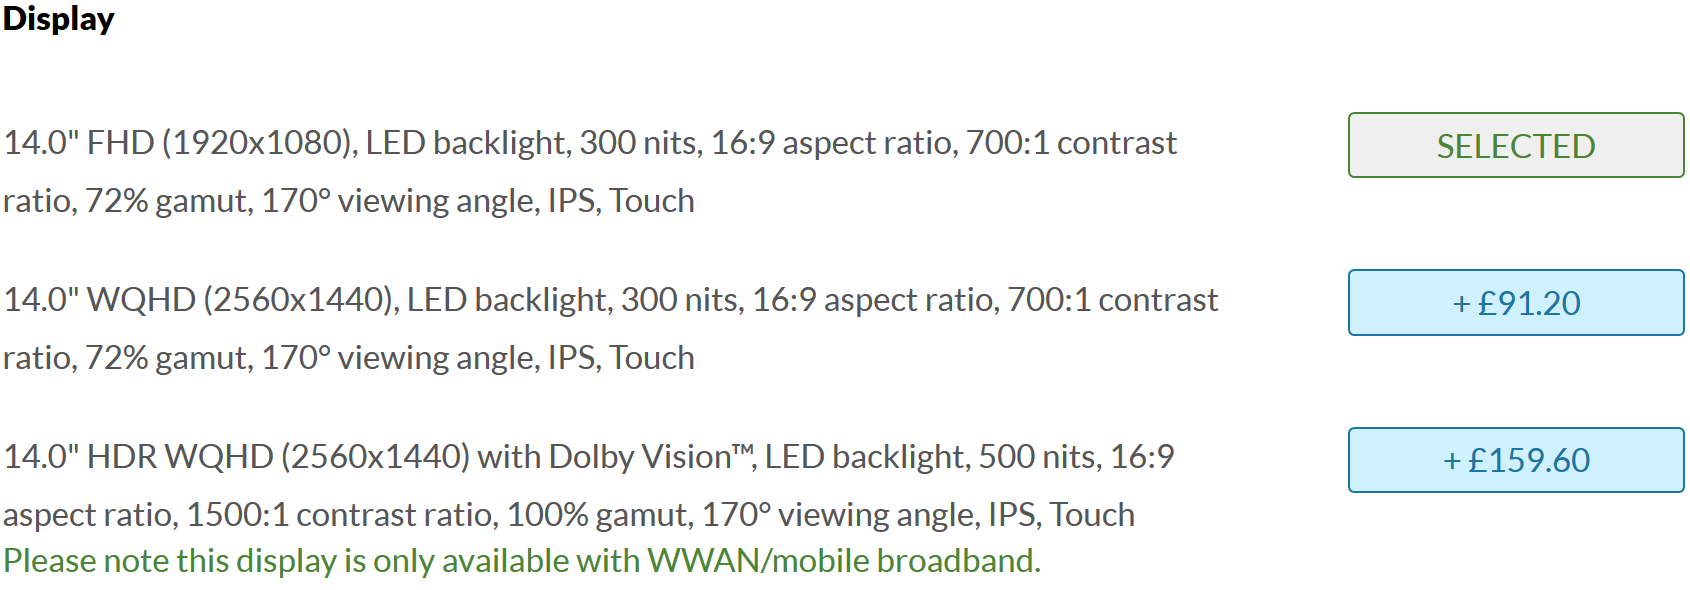
\includegraphics[width=\linewidth]{thinkpad-x1-yoga-display}}\only<2|handout:0>{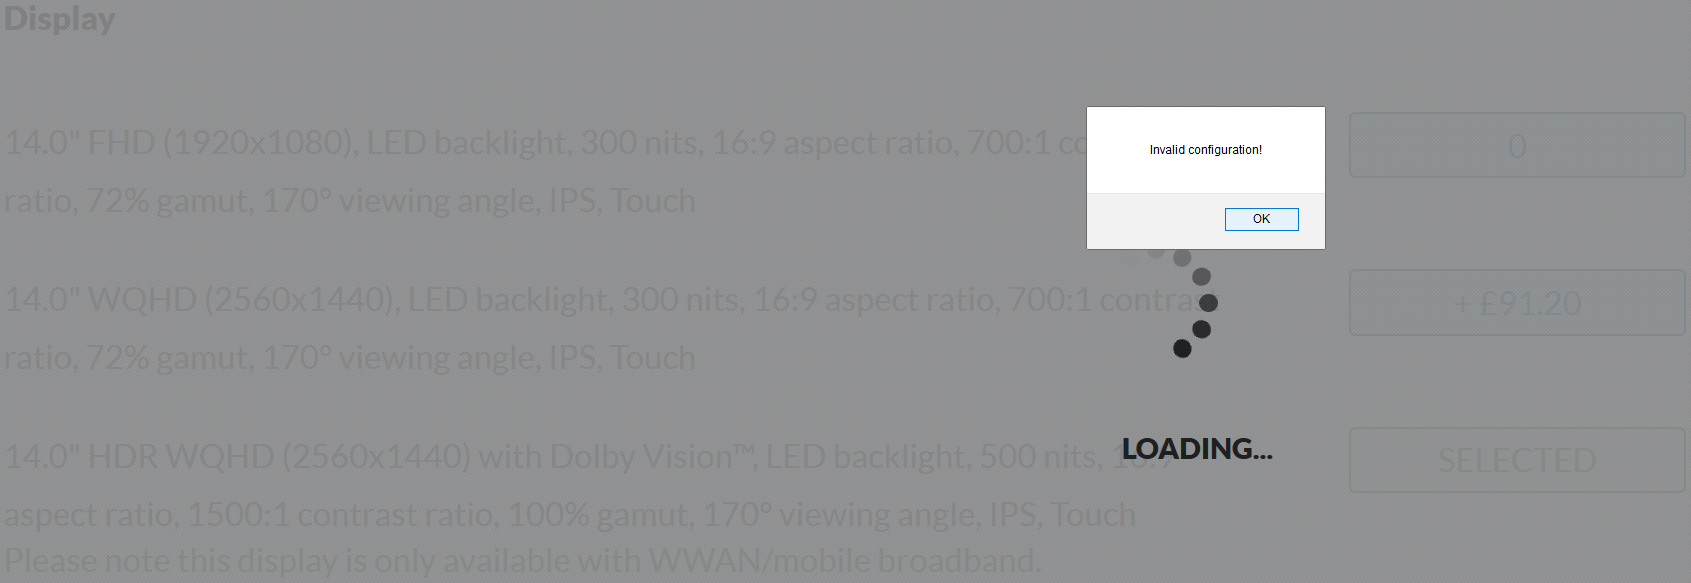
\includegraphics[width=\linewidth]{thinkpad-x1-yoga-display-invalidconf}}}}
\end{frame}

\begin{frame}{\insertsubsection}
	\partofpage{70}{\myexampletight{Thomas Still Configuring a Notebook}{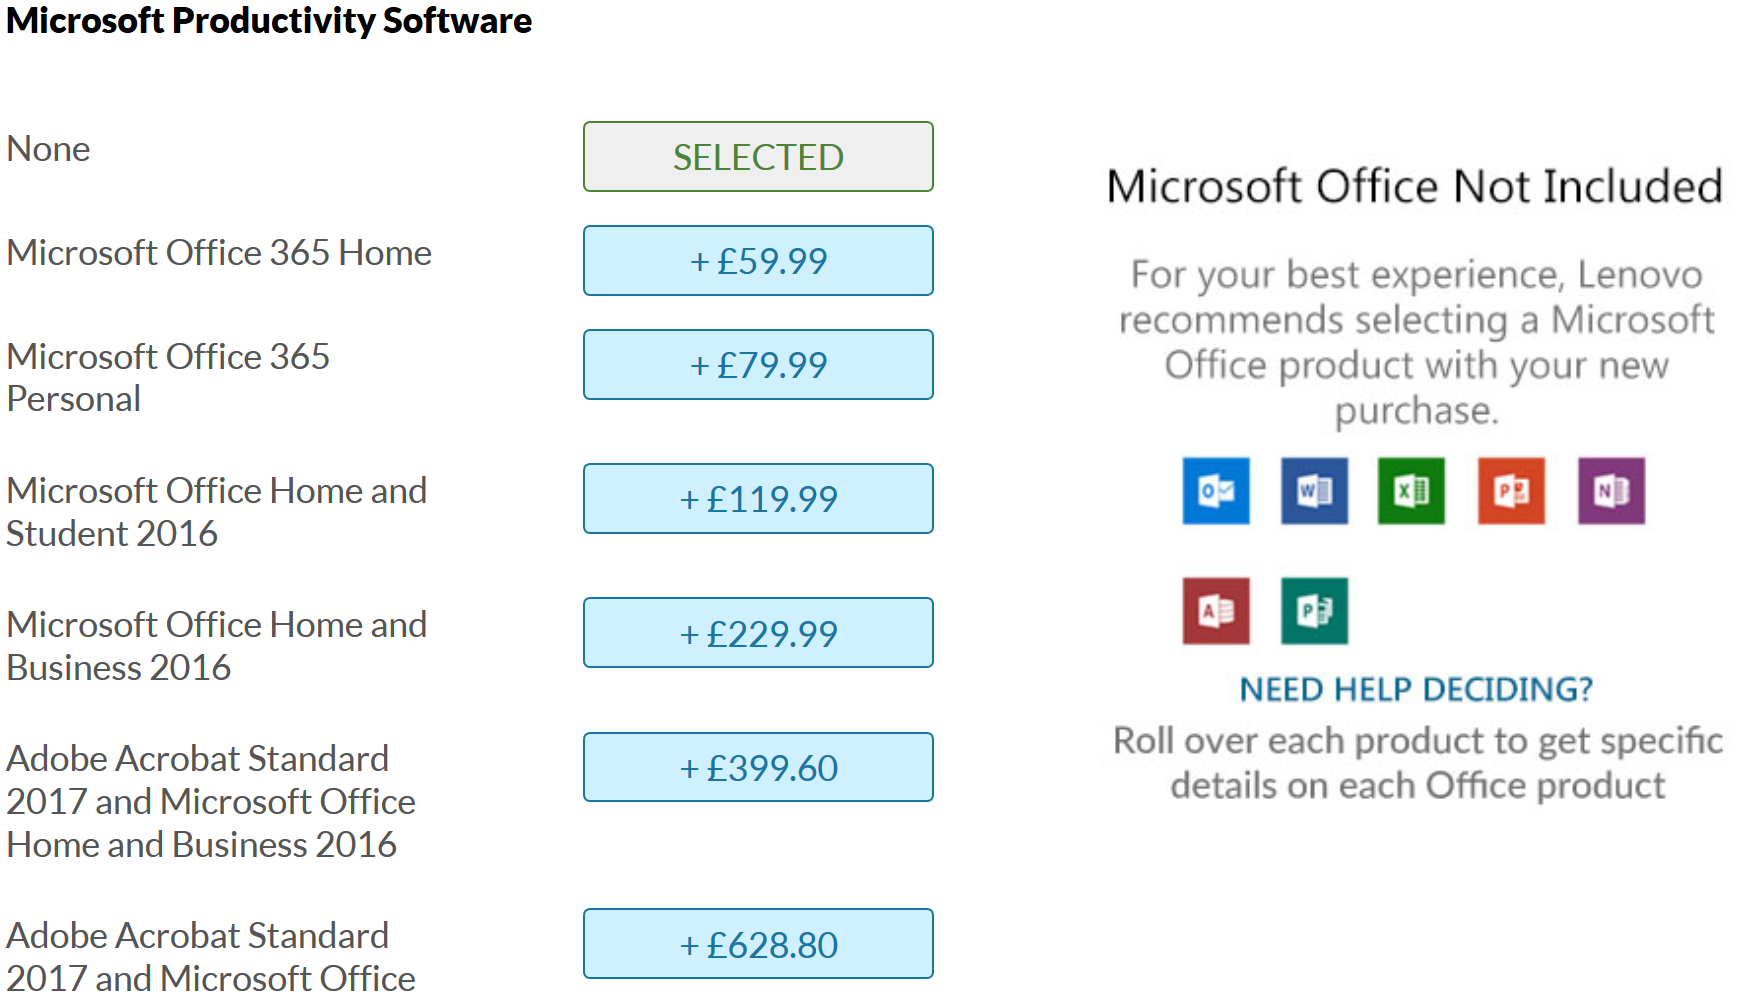
\includegraphics[width=\linewidth]{thinkpad-x1-yoga-office}}}
\end{frame}

\begin{frame}{\insertsubsection}
	~\hfill\partofpage{60}{\myexampletight{Thomas Configuring a Car}{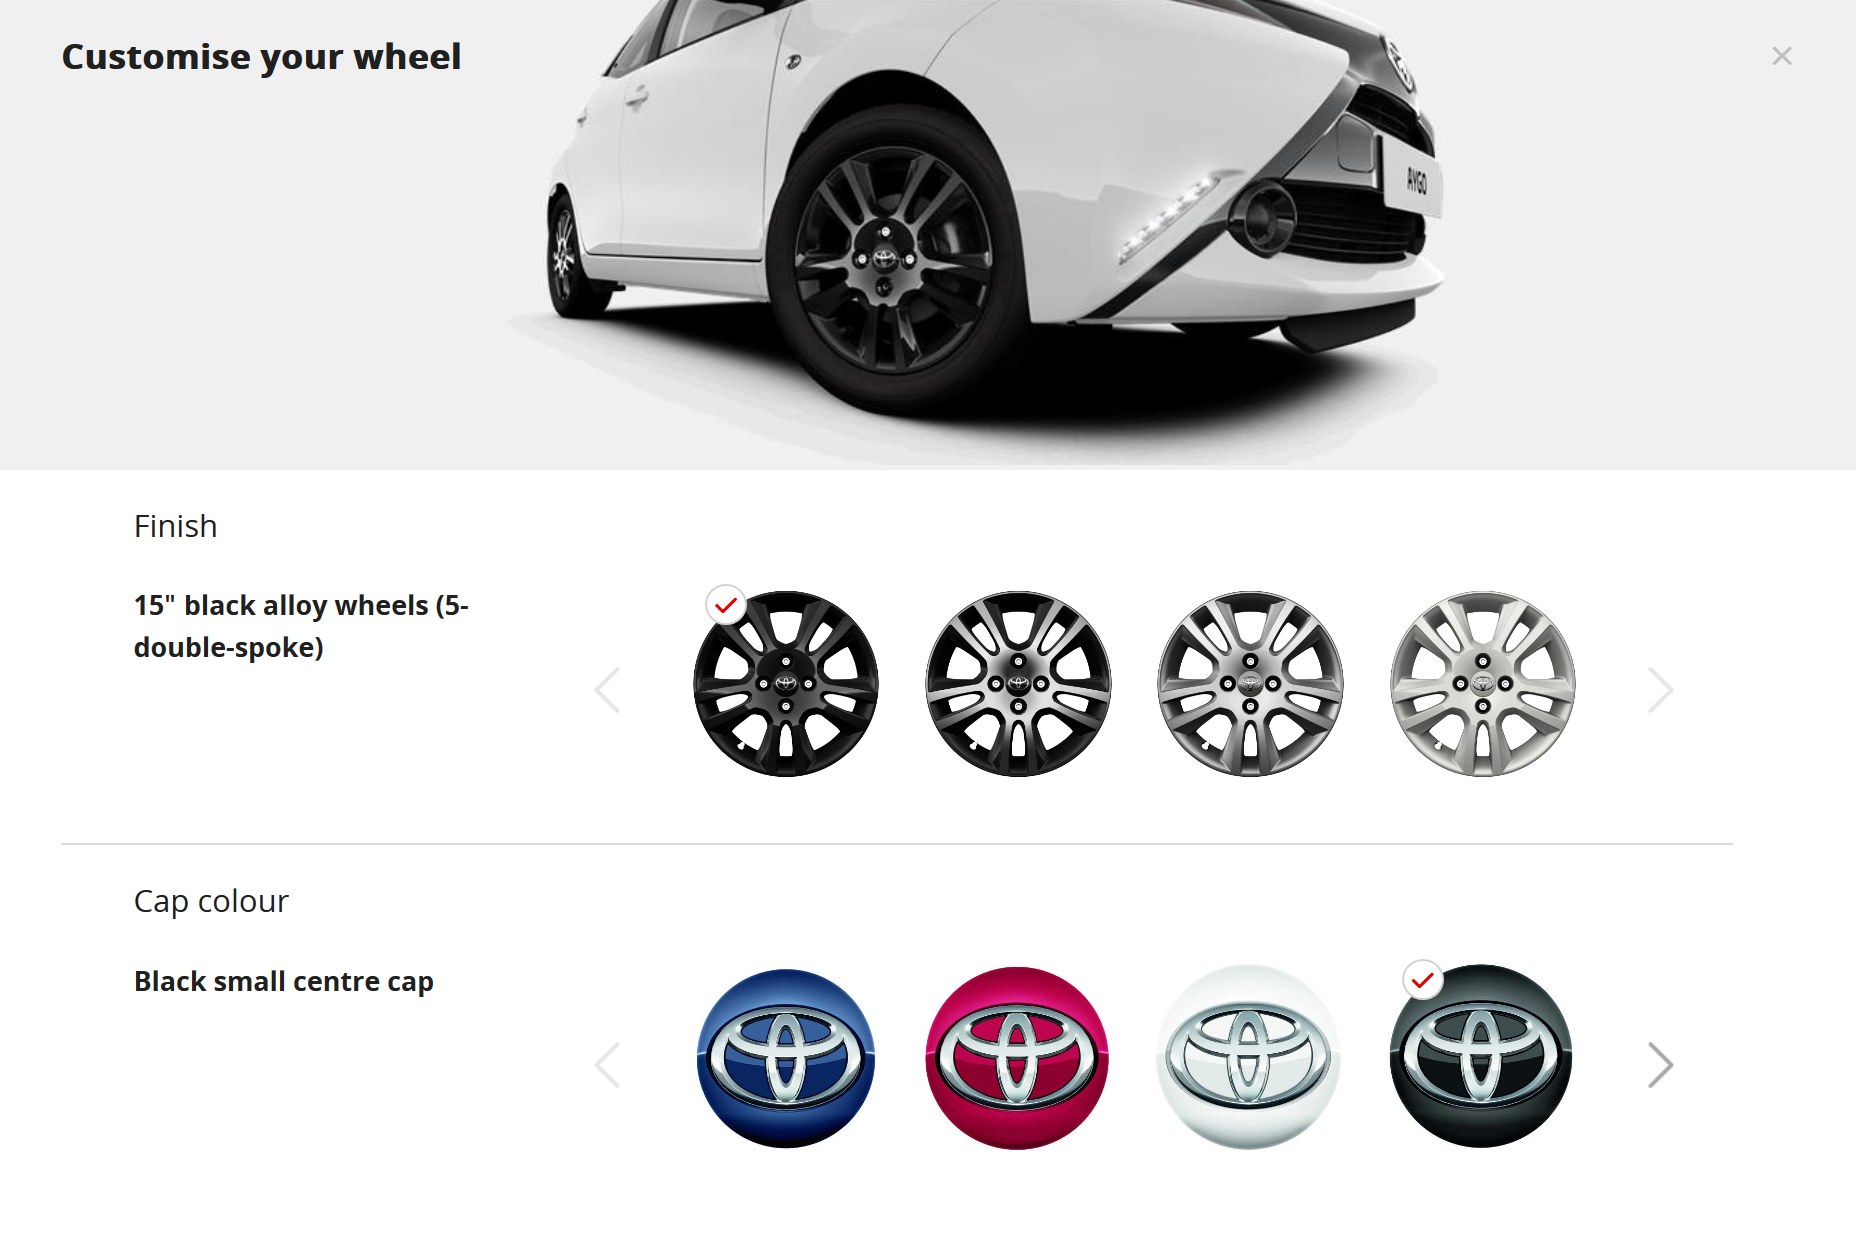
\includegraphics[width=\linewidth]{toyota-aygo-wheels}}}
\end{frame}

\begin{frame}{\insertsubsection}
	~\hfill\partofpage{60}{\myexampletight{Thomas Configuring a Car with a Weird Price}{\centering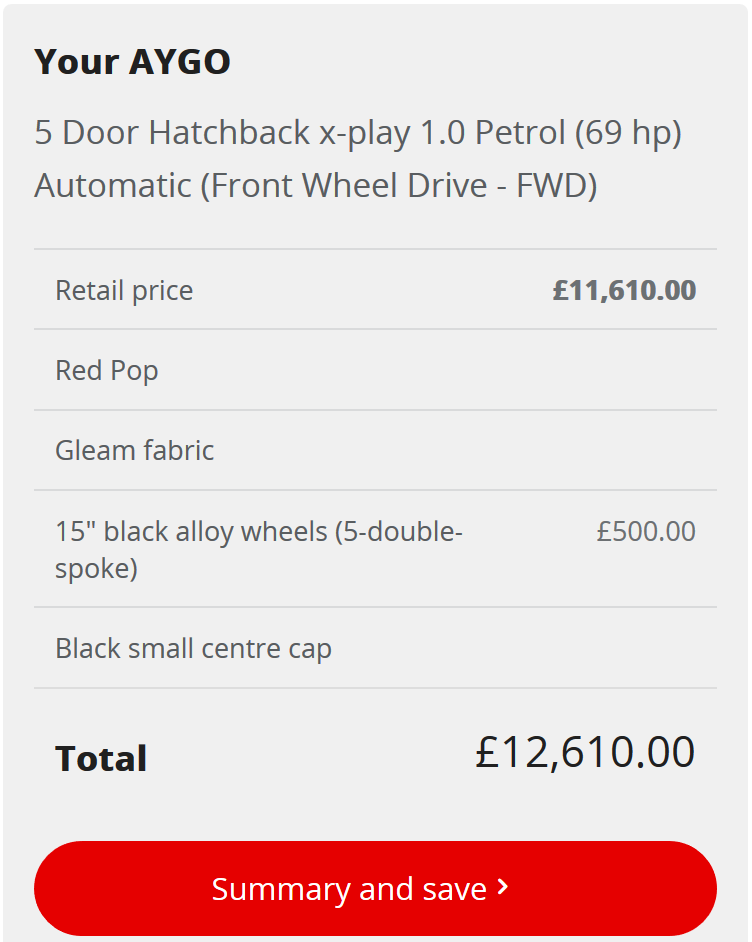
\includegraphics[width=.55\linewidth]{toyota-aygo-costs}}}
\end{frame}

\begin{frame}{\insertsubsection}
	~\hfill\partofpage{60}{\myexampletight{Thomas Configuring a Car with 8 Wheels!}{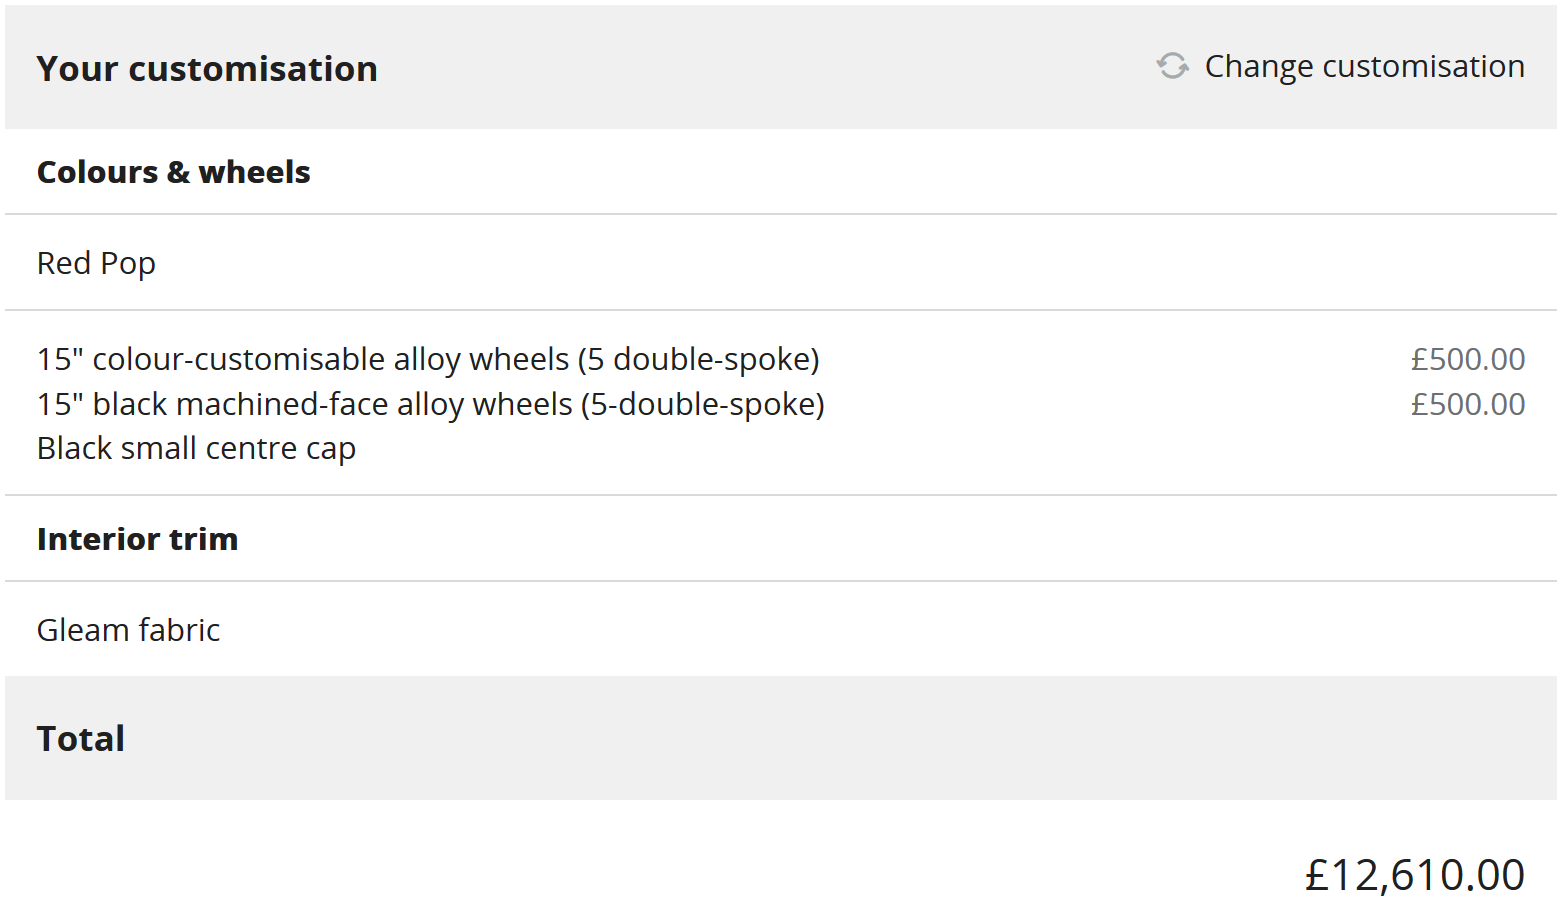
\includegraphics[width=\linewidth]{toyota-aygo-costs3}}}
\end{frame}

\begin{frame}{\insertsubsection}
	\partofpage{70}{\myexampletight{Thomas Configuring a German Car}{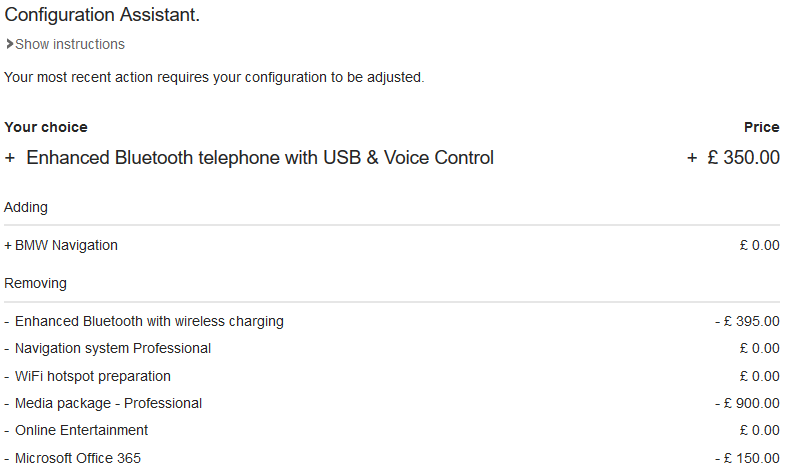
\includegraphics[width=\linewidth]{bmw-series1-confassistant-bluetooth}}}
\end{frame}

\subsection{Feature Modeling} % syntax + semantics

\newcommand{\dbmpl}{
	\myexampletight{A Database Management Product Line \todo{Feature Model?}}{
		\centering
		\featureDiagramDbmgmt\\
		$\mathit{Transactions} \pimplies \mathit{Put} \por \mathit{Delete}$

		\featureDiagramLegend
	}
}

\begin{frame}{\insertsubsection\ \mytitlesource{\fospl}}
	\leftorright{
		\dbmpl
	}{
		\mydefinition{Feature Diagram \todo{vs model?}}{
			\begin{itemize}
				\item hierarchy of features
				\item dependencies between features modeled by tree and cross-tree constraints
				\item \emph{tree constraints}: defined by the hierarchy
				\item \emph{cross-tree constraints}: propositional formulas over features
				\item \emph{concrete features} have an implementation
				\item \emph{abstract features} are used to group other features
			\end{itemize}
		}
	}
\end{frame}

\begin{frame}{\insertsubsection\ \mytitlesource{\fospl}}
	\leftorright{
		\dbmpl
	}{
		\mydefinition{Tree Constraints}{
			\begin{itemize}
				\item each feature requires its parent
				\item an \emph{optional feature} \todo{has no further constraints}{can be (de-)selected freely when its parent is selected}
				\item a \emph{mandatory feature} is required by its parent
				\item \emph{or group}: at least one feature must be selected when the parent is selected
				\item \emph{alternative group}: exactly one feature must be selected when the parent is selected
			\end{itemize}
		}
		\mydefinition{Cross-Tree Constraints}{
			\begin{itemize}
				\item a list of propositional formulas expressing further dependencies between features
			\end{itemize}
		}
	}
\end{frame}

\begin{frame}{\insertsubsection\ \mytitlesource{\fospl}}
	\leftorright{
		\todo{other feature diagram example(s) which shows off how notation can also be used}
	}{
		\mydefinition{Remarks on Notation}{
			\begin{itemize}
				\item abstract/concrete features can be assigned arbitrarily
    			\item groups can be used anywhere
				\item directly below groups, no optional/mandatory markers are allowed
			\end{itemize}
		}
	}
\end{frame}

\lessonslearned{
	\item Motivation for mass customization
	\item Software product lines, features, dependencies between features, configurators
	\item Feature models: abstract and concrete features, tree and cross-tree constraints
	\item Tree constraints: optional, mandatory, or group, alternative group
	\item Feature modeling in practice
	\item Further Reading: \fospl, Chapter~1 Software Product Lines and Section~2.3 Feature Modeling
}{
	\item Sketch a feature model that has 9 valid configurations (pen and paper preferred)
	\item Upload your feature model to Moodle
	\item Inspect whether other submitted solutions are syntactically correct and have the right number of configurations
	\\\hfill%\qrcode{https://moodle.uni-ulm.de/mod/moodleoverflow/discussion.php?d=4494} % TODO in 2023 update link
}{}
